% ============================================================================
%  Measuring the Global AI Startup Ecosystem -- a short methods note
%
%  Self-contained: compiles with pdflatex alone (no bibtex, no figures).
%  This is the plain-language companion to main.tex. Every number here is
%  carried over from that paper; nothing new is claimed.
% ============================================================================
\documentclass[11pt]{article}

\usepackage[margin=1.15in]{geometry}
\usepackage{booktabs}
\usepackage{amsmath,amssymb}
\usepackage[hidelinks]{hyperref}
\usepackage{natbib}
\usepackage{enumitem}
\usepackage{graphicx}
\usepackage{tikz}
\usetikzlibrary{positioning, arrows.meta, calc}

\title{\textbf{Measuring the Global AI Startup Ecosystem}\\[0.35em]
\large A Short Note on the Dataset, the Evidence, and Its Limits}

\author{Alastair Page \and Jihwan (Victor) Park\thanks{%
Tobin Center for Economic Policy, Yale University. We thank Professor Song Ma
for supervising this research and for framing the broader agenda on artificial
intelligence and the global startup ecosystem. Errors are ours.
Correspondence: \texttt{victorjhp11@gmail.com}.}}

\date{August 2026}

\begin{document}
\maketitle

\begin{abstract}
\noindent
This note asks how artificial intelligence is changing which companies are
founded, where they appear, and what they build. The central obstacle is
measurement: most startup evidence comes from a few commercial company
databases, and those databases observe firms selectively. We explain how we
built a dataset of $988{,}576$ firms from six source classes, how we labelled
firms as AI-related, and how we validated the resulting measurements. Three
results stand out. AI's share of newly founded firms rises from $3.0\%$ in 2000
to $59.0\%$ in 2025. Firms missed by the commercial databases are about twice
as likely to be AI-related. Finally, when a language model is asked to infer
missing company details, it fills gaps with prior beliefs rather than
evidence---which is why our final pipeline allows model extraction only from
text we already hold.
\end{abstract}

\medskip
\noindent\textbf{Keywords:} artificial intelligence, entrepreneurship,
measurement, coverage bias

% ============================================================================
\section{The question, and why it is hard}
% ============================================================================

Artificial intelligence may change who starts companies and what those
companies do \citep{fossen2024ai}. Early evidence suggests that generative AI
raises worker productivity \citep{brynjolfsson2023genai} and may already be
shifting entry decisions \citep{bena2025prompted}. Studying those changes at
the firm level requires a simple object that is surprisingly hard to obtain: a
set of firms we can observe.

Most empirical work on entrepreneurship relies on commercial startup databases.
Those databases are valuable, but they are not population registers. A firm
enters when there is a reason to record it: a financing round, a press mention,
an acquisition, or a founder-submitted profile. \citet{dalle2017crunchbase}
document this issue for one widely used database and show that coverage is
uneven in ways that can affect research conclusions.

So a rise in ``AI firms founded'' can mean two very different things:

\begin{enumerate}[leftmargin=1.4em, itemsep=2pt]
  \item more AI firms are actually being founded, or
  \item the databases became better at observing them.
\end{enumerate}

\noindent
We therefore collect firms from sources with \emph{different} inclusion
mechanisms---funders, code hosts, accelerator pages, venture portfolios, and
launch directories. That lets us compare firms recorded by commercial
databases with firms those databases never picked up. The difference between
the two is not a nuisance to be waved away; it is one of the quantities we
measure.

% ============================================================================
\section{Where the firms come from}
% ============================================================================

We combine six source classes (Table~\ref{tab:sources}). Their value is not
only that they add more firms; it is that each source observes a different
part of the startup ecosystem.

\begin{table}[htbp]
\centering\small
\caption{Sources and their contribution. Counts overlap; the union after
merging duplicates is $988{,}576$.}
\label{tab:sources}
\begin{tabular}{@{}p{3.5cm}p{5.4cm}r@{}}
\toprule
\textbf{Source} & \textbf{What it records} & \textbf{Firms} \\
\midrule
Commercial database A & general startup register & $650{,}200$ \\
Commercial database B & venture-financing register & $281{,}395$ \\
Public funder registries & U.S.\ federal small-business awards; national
health and science agencies; E.U.\ framework programme & $9{,}931$ \\
Open-source code host & organisations found by topic and keyword search &
$31{,}909$ \\
Portfolios and programmes & accelerators, university venture programmes,
venture portfolios & $27{,}330$ \\
General web collection & launch directories, national ecosystem sites &
$1{,}010$ \\
\midrule
\textbf{Total (after merging)} & & $\mathbf{988{,}576}$ \\
\bottomrule
\end{tabular}
\end{table}

The first two rows are the conventional evidence base. The remaining four rows
are designed to reveal firms the commercial databases may miss. A company that
wins a federal research award, for example, appears in a public registry
whether or not it has raised venture capital or received press coverage.

% ============================================================================
\section{How we built the dataset}
% ============================================================================

\subsection{Collecting}

Sources arrive in many formats, so the collection system chooses one of five
strategies for each source: download a bulk file, call a documented endpoint,
run a source-specific parser ($36$ are implemented), use a bounded
tool-using language-model agent, or suspend the source. The agent is capped at
$10$ reasoning steps, $12$ plain page fetches, and $8$ browser-rendered fetches
per site. When it succeeds, it writes a reusable extraction rule, allowing the
next run to return to a cheaper strategy.

Strategies are updated from observed outcomes rather than hand-tuned decisions
(Figure~\ref{fig:collection}).

\begin{figure}[htbp]
\centering
\resizebox{\textwidth}{!}{%
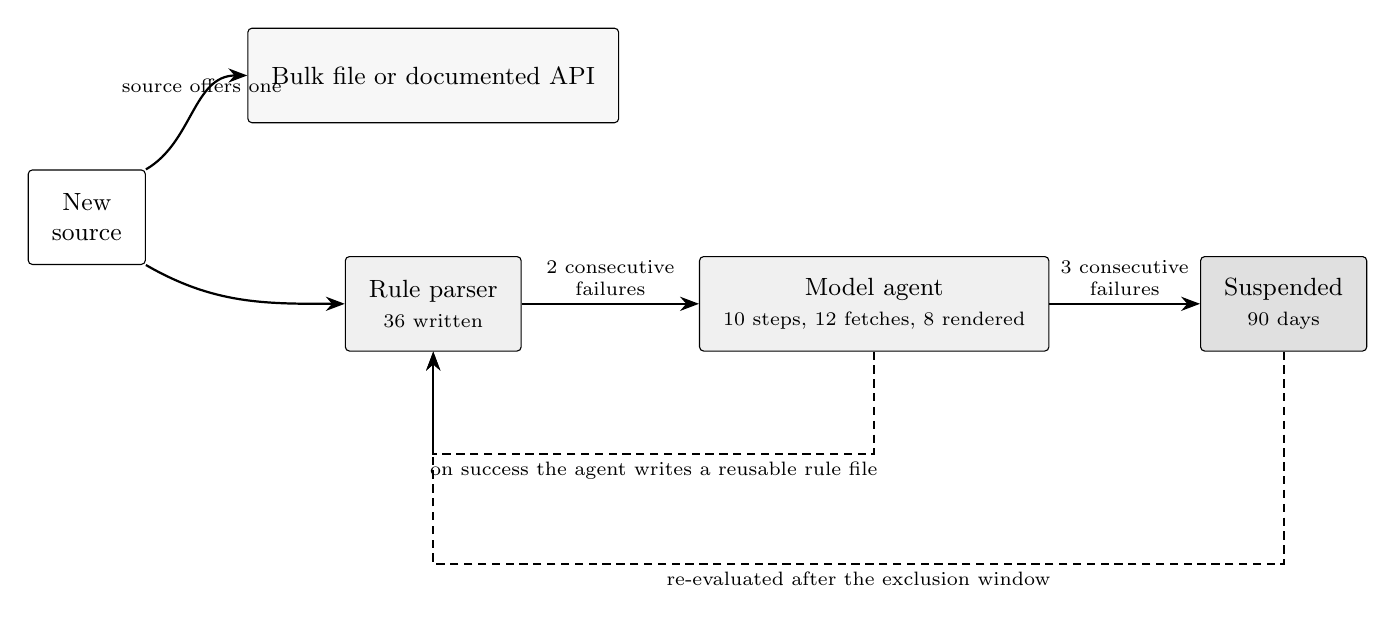
\begin{tikzpicture}[
  box/.style   = {draw, align=center, font=\small, rounded corners=1.5pt,
                  minimum height=12mm, inner xsep=3mm},
  cheap/.style = {box, fill=black!3},
  work/.style  = {box, fill=black!6},
  stop/.style  = {box, fill=black!12},
  flow/.style  = {-{Stealth[length=2.4mm]}, thick},
  back/.style  = {-{Stealth[length=2.4mm]}, thick, densely dashed},
  lbl/.style   = {font=\scriptsize, align=center, inner sep=2.5pt},
]

% --- nodes ---------------------------------------------------------------
\node[box]   (src)   at (0,0)       {New\\source};
\node[cheap] (api)   at (4.4,1.8)   {Bulk file or documented API};
\node[work]  (rule)  at (4.4,-1.1)  {Rule parser\\{\scriptsize 36 written}};
\node[work]  (agent) at (10.0,-1.1) {Model agent\\{\scriptsize 10 steps, 12 fetches, 8 rendered}};
\node[stop]  (susp)  at (15.2,-1.1) {Suspended\\{\scriptsize 90 days}};

% --- entry ---------------------------------------------------------------
\draw[flow] (src.north east) to[out=30,in=180]
     node[lbl,above,pos=0.6] {source offers one} (api.west);
\draw[flow] (src.south east) to[out=-30,in=180] (rule.west);

% --- escalation ----------------------------------------------------------
\draw[flow] (rule) -- node[lbl,above] {2 consecutive\\failures} (agent);
\draw[flow] (agent) -- node[lbl,above] {3 consecutive\\failures} (susp);

% --- feedback ------------------------------------------------------------
\coordinate (a1) at ($(agent.south)+(0,-1.3)$);
\coordinate (r1) at ($(rule.south)+(0,-1.3)$);
\draw[back] (agent.south) -- (a1)
     -- node[lbl,below] {on success the agent writes a reusable rule file} (r1)
     -- (rule.south);

\coordinate (s2) at ($(susp.south)+(0,-2.7)$);
\coordinate (r2) at ($(rule.south)+(0,-2.7)$);
\draw[back] (susp.south) -- (s2)
     -- node[lbl,below] {re-evaluated after the exclusion window} (r2)
     -- (rule.south);

\end{tikzpicture}}
\caption{How one source gets collected. Cost rises from left to right, so the
expensive strategy is reached only where the cheap ones have already failed, and
a successful agent run leaves behind a rule file that returns the source to the
cheap path. A parser is also escalated when it returns fewer than $20$ records
from a page that shows pagination controls, which catches a scraper that is
technically succeeding while reading only the first page. A zero-record run also
counts as a failure, preventing a silently broken parser from looking healthy.
Sources that succeed are not revisited for seven days.}
\label{fig:collection}
\end{figure}

The yield is informative precisely because it is uneven. Of $410$ sites
attempted, $220$ ($53.7\%$) ever produced a successful extraction. Among
successful sites, the mean yield is $22.9$ records, the median is $6$, and the
maximum is $814$. Projecting from the mean alone therefore overstates the
available data by roughly a factor of four. This is a practical lesson from the
project: source lists record attempts, not necessarily usable data.

\subsection{Merging records that name the same firm}

The same company often appears in several sources under slightly different
names. Deciding when two records refer to one firm is record linkage, a problem
with a long methodological literature \citep{abramitzky2021linking}.

Our production rule is deliberately conservative. Each record receives one key:
its registrable web domain, if available; otherwise a normalised version of its
name. Two records are merged only when their keys are equal. A blocklist
prevents code hosts, documentation sites, and social platforms from being
treated as company domains, which would otherwise merge unrelated firms that
share a hosting provider.

This conservative rule still exposed an important defect. The name normaliser
strips common corporate tokens, including ``AI.'' In this setting, that token
can distinguish a new AI firm from an older namesake. No matching threshold can
repair a pipeline that deletes the distinguishing word before matching begins.

\subsection{Deciding whether a firm is ``AI''}

A firm is labelled AI-related if \emph{any} of four signals fires:

\begin{equation}
\label{eq:ai}
A_i \;=\; \mathbb{1}\big[\,
\underbrace{t_i}_{\text{vendor tag}} \;\vee\;
\underbrace{a_i \ge 0.5}_{\text{keyword score}} \;\vee\;
\underbrace{m_i}_{\text{AI mentioned in text}} \;\vee\;
\underbrace{\ell_i}_{\text{model verdict}}
\,\big].
\end{equation}

The signals are evaluated from cheapest to most expensive, so the model is used
only when cheaper evidence is insufficient. Language-model classification is
now common in economics \citep{dell2025deep}; our main caution is not that the
model cannot classify text, but that the available signals differ sharply
across sources.

Two properties of \eqref{eq:ai} shape everything downstream.

\textbf{The signals are not equally available.} Vendor tags cover $7.0\%$ of
database-A firms, $0.7\%$ of database-B firms, and $0.0\%$ of firms found
outside both. Model verdicts were run on $98.8\%$ of database B but only
$2.3\%$ of the unlisted layer. Only the two description-derived signals are
computed identically for every firm. Cross-population comparisons must
therefore either use the full union and acknowledge the asymmetry, or restrict
to signals available everywhere. We report both.

\textbf{The keyword score does not transfer across sources.} Database-B records
carry no topic tags and have short descriptions, so the highest score they can
reach is $0.3$---below the $0.5$ threshold by construction. Under a
tag-or-score definition database B appears $1.3\%$ AI; under the full union it
is $10.7\%$. A threshold calibrated on one source had silently excluded
$281{,}395$ firms in another. We found the problem by checking each source's
attainable score range, a diagnostic we now treat as routine.

\subsection{Filling in missing fields}

Many firms lack a founding year, country, or industry. We enrich these fields
under a strict rule about \emph{where a value may come from}:

\begin{enumerate}[leftmargin=2.2em, itemsep=2pt]
  \item[$T_1$] an official registry (free, checkable);
  \item[$T_2$] a document we fetched ourselves;
  \item[$T_3$] a language model reading a text we already hold;
  \item[$T_4$] a language model recalling a fact from its own memory ---
        \textbf{prohibited}.
\end{enumerate}

Every stored value keeps its tier and its source alongside it, so any analysis
can filter by origin. Section~\ref{sec:checks} explains what happened when
$T_4$ was briefly allowed, and why provenance made the resulting contamination
removable rather than invisible.

% ============================================================================
%  Findings section for short.tex
%  This file is a TeX fragment, intended to be included with:
%  % ============================================================================
%  Findings section for short.tex
%  This file is a TeX fragment, intended to be included with:
%  % ============================================================================
%  Findings section for short.tex
%  This file is a TeX fragment, intended to be included with:
%  \input{findings_global_formation}
% ============================================================================

\section{Findings: Global AI Startup Formation}
\label{sec:findings_global_formation}

The main descriptive pattern is simple: AI has become a much larger share of
new startup formation. The harder part is interpretation. Recent founding
cohorts are still being indexed, so raw counts understate recent formation.
For that reason, the formation result is stated primarily as a \emph{share of
observed firms founded in the same year}, not as the raw number of AI firms.

\subsection{AI's share of new firms rises sharply}

In the commercial population, where founding years are nearly complete, the AI
share rises from $3.0\%$ in 2000 to $10.6\%$ in 2015, $18.9\%$ in 2021, and
$59.0\%$ in 2025 (Table~\ref{tab:formation_selected_years}). The largest break
in the series is between the 2022 and 2023 founding cohorts, when the AI share
jumps from $25.5\%$ to $43.5\%$. That timing is consistent with the public
release of consumer generative AI in late 2022, but we do not interpret the
jump causally. The same cohorts are also affected by indexing lag, and the
paper does not have a design that separates the technology shock from the
change in observability.

\begin{table}[htbp]
\centering\small
\caption{AI share of observed startup formation, selected founding cohorts.
The sample is the commercial population, where founding years are nearly
complete.}
\label{tab:formation_selected_years}
\begin{tabular}{@{}rrrr@{}}
\toprule
\textbf{Founded year} & \textbf{Observed firms} & \textbf{AI firms} &
\textbf{AI share} \\
\midrule
2000 & $28{,}963$ & $874$ & $3.0\%$ \\
2010 & $41{,}513$ & $1{,}996$ & $4.8\%$ \\
2015 & $54{,}150$ & $5{,}764$ & $10.6\%$ \\
2018 & $50{,}542$ & $8{,}038$ & $15.9\%$ \\
2021 & $35{,}978$ & $6{,}812$ & $18.9\%$ \\
2022 & $22{,}800$ & $5{,}818$ & $25.5\%$ \\
2023 & $17{,}947$ & $7{,}812$ & $43.5\%$ \\
2024 & $10{,}562$ & $5{,}534$ & $52.4\%$ \\
2025 & $2{,}531$ & $1{,}492$ & $59.0\%$ \\
\bottomrule
\end{tabular}
\end{table}

The count series tells a different story. The observed number of AI firms peaks
in 2018 at $8{,}038$ and falls after that. We do not read this as a decline in
AI entrepreneurship. The total observed denominator falls from $54{,}150$ firms
in the 2015 cohort to $2{,}531$ in 2025, because recent firms have not yet had
time to enter commercial registers. The useful fact is therefore not that
observed AI counts fall after 2018, but that AI's share continues to rise even
as the recent denominator becomes incomplete.

\subsection{The trend is not driven by one source}

The rise appears in both commercial databases. Database A rises from $2.7\%$
AI in the 2000 cohort to $63.7\%$ in 2025. Database B rises from $3.6\%$ to
$58.3\%$ over the same window. The levels differ somewhat, but the direction
does not. This matters because a trend visible in only one database could
reflect a vendor-specific tagging or coverage decision. Here, both sources
show the same broad movement.

\subsection{The trend survives a stricter selection rule}

Recent cohorts are not only smaller; they are also more selected. A young firm
is especially likely to appear in a commercial database if it has already done
something visible, such as raising financing. If AI firms are more likely to be
visible early, the rising AI share could partly reflect selection into the
database rather than startup formation itself.

We check this by holding the selection rule fixed: among firms with recorded
financing, the AI share still rises from $5.9\%$ in 2005 to $15.6\%$ in 2015,
$22.0\%$ in 2021, and $68.3\%$ in 2025. The level is higher because financed
firms are more AI-intensive, but the time pattern remains. This does not solve
all selection problems, but it rules out the simplest concern that the trend is
only an artifact of looser recent coverage.

\subsection{Commercial databases miss AI-heavy firms}

The formation series above uses the commercial population because it has the
founding-year metadata needed for a time trend. The broader dataset also
reveals what those commercial sources miss. Firms found outside both
commercial databases are $23.8\%$ AI-related, compared with $12.4\%$ in
database A and $10.7\%$ in database B. The unlisted layer is therefore roughly
twice as AI-intensive as the conventional evidence base.

We do not use the unlisted layer to extend the time series, because its
founding-year coverage is thin. Its value is different: it shows the direction
of coverage bias. If the firms missing from commercial databases are more
likely to be AI-related, then commercial-only studies will understate AI entry.
Section~\ref{sec:checks} tests whether that gap survives alternative AI
definitions, source exclusions, independent labels, and classifier-error
correction.

\subsection{The global pattern is broad growth with cautious geography}

AI intensity rises across every major region we can measure. Between the
2010--2016 and 2020--2025 cohorts, North America's AI share rises from $9.1\%$
to $29.2\%$, Europe's from $7.3\%$ to $21.4\%$, East Asia's from $12.3\%$ to
$25.1\%$, and South and Southeast Asia's from $7.2\%$ to $18.2\%$. Among large
country samples, recent AI intensity is highest in Israel ($37.2\%$), the
United States ($29.4\%$), China ($28.5\%$), Canada ($27.3\%$), and South Korea
($26.1\%$).

The concentration series is more delicate. Through 2017, AI entrepreneurship
appears to become more geographically dispersed: the number of observed
countries with AI firms rises from $59$ in 2000 to $103$ in 2017, and the U.S.\
share of observed AI firms falls from $41.3\%$ to $36.8\%$. After 2020 the
series reverses sharply, with the U.S.\ reaching $85.0\%$ of observed AI firms
in the 2025 cohort. We treat that reversal as a coverage warning rather than a
substantive geography result, because the newest non-U.S.\ firms are indexed
more slowly.

\subsection{AI growth is broad across sectors}

The sector pattern is also one of broad intensification rather than a single
vertical driving the result. Data and analytics rises from $35.9\%$ AI in the
2010--2016 cohort to $71.4\%$ in 2020--2025. Biotech and pharma rises from
$23.2\%$ to $60.0\%$, software and IT from $9.5\%$ to $29.3\%$, and healthcare
from $8.9\%$ to $26.6\%$. Lower-intensity sectors also rise: food and agtech,
consumer and lifestyle, and e-commerce and retail all more than double their
AI shares. The ordering changes less than the levels. Sectors that were already
AI-intensive remain near the top, while nearly every sector moves upward.

% ============================================================================

\section{Findings: Global AI Startup Formation}
\label{sec:findings_global_formation}

The main descriptive pattern is simple: AI has become a much larger share of
new startup formation. The harder part is interpretation. Recent founding
cohorts are still being indexed, so raw counts understate recent formation.
For that reason, the formation result is stated primarily as a \emph{share of
observed firms founded in the same year}, not as the raw number of AI firms.

\subsection{AI's share of new firms rises sharply}

In the commercial population, where founding years are nearly complete, the AI
share rises from $3.0\%$ in 2000 to $10.6\%$ in 2015, $18.9\%$ in 2021, and
$59.0\%$ in 2025 (Table~\ref{tab:formation_selected_years}). The largest break
in the series is between the 2022 and 2023 founding cohorts, when the AI share
jumps from $25.5\%$ to $43.5\%$. That timing is consistent with the public
release of consumer generative AI in late 2022, but we do not interpret the
jump causally. The same cohorts are also affected by indexing lag, and the
paper does not have a design that separates the technology shock from the
change in observability.

\begin{table}[htbp]
\centering\small
\caption{AI share of observed startup formation, selected founding cohorts.
The sample is the commercial population, where founding years are nearly
complete.}
\label{tab:formation_selected_years}
\begin{tabular}{@{}rrrr@{}}
\toprule
\textbf{Founded year} & \textbf{Observed firms} & \textbf{AI firms} &
\textbf{AI share} \\
\midrule
2000 & $28{,}963$ & $874$ & $3.0\%$ \\
2010 & $41{,}513$ & $1{,}996$ & $4.8\%$ \\
2015 & $54{,}150$ & $5{,}764$ & $10.6\%$ \\
2018 & $50{,}542$ & $8{,}038$ & $15.9\%$ \\
2021 & $35{,}978$ & $6{,}812$ & $18.9\%$ \\
2022 & $22{,}800$ & $5{,}818$ & $25.5\%$ \\
2023 & $17{,}947$ & $7{,}812$ & $43.5\%$ \\
2024 & $10{,}562$ & $5{,}534$ & $52.4\%$ \\
2025 & $2{,}531$ & $1{,}492$ & $59.0\%$ \\
\bottomrule
\end{tabular}
\end{table}

The count series tells a different story. The observed number of AI firms peaks
in 2018 at $8{,}038$ and falls after that. We do not read this as a decline in
AI entrepreneurship. The total observed denominator falls from $54{,}150$ firms
in the 2015 cohort to $2{,}531$ in 2025, because recent firms have not yet had
time to enter commercial registers. The useful fact is therefore not that
observed AI counts fall after 2018, but that AI's share continues to rise even
as the recent denominator becomes incomplete.

\subsection{The trend is not driven by one source}

The rise appears in both commercial databases. Database A rises from $2.7\%$
AI in the 2000 cohort to $63.7\%$ in 2025. Database B rises from $3.6\%$ to
$58.3\%$ over the same window. The levels differ somewhat, but the direction
does not. This matters because a trend visible in only one database could
reflect a vendor-specific tagging or coverage decision. Here, both sources
show the same broad movement.

\subsection{The trend survives a stricter selection rule}

Recent cohorts are not only smaller; they are also more selected. A young firm
is especially likely to appear in a commercial database if it has already done
something visible, such as raising financing. If AI firms are more likely to be
visible early, the rising AI share could partly reflect selection into the
database rather than startup formation itself.

We check this by holding the selection rule fixed: among firms with recorded
financing, the AI share still rises from $5.9\%$ in 2005 to $15.6\%$ in 2015,
$22.0\%$ in 2021, and $68.3\%$ in 2025. The level is higher because financed
firms are more AI-intensive, but the time pattern remains. This does not solve
all selection problems, but it rules out the simplest concern that the trend is
only an artifact of looser recent coverage.

\subsection{Commercial databases miss AI-heavy firms}

The formation series above uses the commercial population because it has the
founding-year metadata needed for a time trend. The broader dataset also
reveals what those commercial sources miss. Firms found outside both
commercial databases are $23.8\%$ AI-related, compared with $12.4\%$ in
database A and $10.7\%$ in database B. The unlisted layer is therefore roughly
twice as AI-intensive as the conventional evidence base.

We do not use the unlisted layer to extend the time series, because its
founding-year coverage is thin. Its value is different: it shows the direction
of coverage bias. If the firms missing from commercial databases are more
likely to be AI-related, then commercial-only studies will understate AI entry.
Section~\ref{sec:checks} tests whether that gap survives alternative AI
definitions, source exclusions, independent labels, and classifier-error
correction.

\subsection{The global pattern is broad growth with cautious geography}

AI intensity rises across every major region we can measure. Between the
2010--2016 and 2020--2025 cohorts, North America's AI share rises from $9.1\%$
to $29.2\%$, Europe's from $7.3\%$ to $21.4\%$, East Asia's from $12.3\%$ to
$25.1\%$, and South and Southeast Asia's from $7.2\%$ to $18.2\%$. Among large
country samples, recent AI intensity is highest in Israel ($37.2\%$), the
United States ($29.4\%$), China ($28.5\%$), Canada ($27.3\%$), and South Korea
($26.1\%$).

The concentration series is more delicate. Through 2017, AI entrepreneurship
appears to become more geographically dispersed: the number of observed
countries with AI firms rises from $59$ in 2000 to $103$ in 2017, and the U.S.\
share of observed AI firms falls from $41.3\%$ to $36.8\%$. After 2020 the
series reverses sharply, with the U.S.\ reaching $85.0\%$ of observed AI firms
in the 2025 cohort. We treat that reversal as a coverage warning rather than a
substantive geography result, because the newest non-U.S.\ firms are indexed
more slowly.

\subsection{AI growth is broad across sectors}

The sector pattern is also one of broad intensification rather than a single
vertical driving the result. Data and analytics rises from $35.9\%$ AI in the
2010--2016 cohort to $71.4\%$ in 2020--2025. Biotech and pharma rises from
$23.2\%$ to $60.0\%$, software and IT from $9.5\%$ to $29.3\%$, and healthcare
from $8.9\%$ to $26.6\%$. Lower-intensity sectors also rise: food and agtech,
consumer and lifestyle, and e-commerce and retail all more than double their
AI shares. The ordering changes less than the levels. Sectors that were already
AI-intensive remain near the top, while nearly every sector moves upward.

% ============================================================================

\section{Findings: Global AI Startup Formation}
\label{sec:findings_global_formation}

The main descriptive pattern is simple: AI has become a much larger share of
new startup formation. The harder part is interpretation. Recent founding
cohorts are still being indexed, so raw counts understate recent formation.
For that reason, the formation result is stated primarily as a \emph{share of
observed firms founded in the same year}, not as the raw number of AI firms.

\subsection{AI's share of new firms rises sharply}

In the commercial population, where founding years are nearly complete, the AI
share rises from $3.0\%$ in 2000 to $10.6\%$ in 2015, $18.9\%$ in 2021, and
$59.0\%$ in 2025 (Table~\ref{tab:formation_selected_years}). The largest break
in the series is between the 2022 and 2023 founding cohorts, when the AI share
jumps from $25.5\%$ to $43.5\%$. That timing is consistent with the public
release of consumer generative AI in late 2022, but we do not interpret the
jump causally. The same cohorts are also affected by indexing lag, and the
paper does not have a design that separates the technology shock from the
change in observability.

\begin{table}[htbp]
\centering\small
\caption{AI share of observed startup formation, selected founding cohorts.
The sample is the commercial population, where founding years are nearly
complete.}
\label{tab:formation_selected_years}
\begin{tabular}{@{}rrrr@{}}
\toprule
\textbf{Founded year} & \textbf{Observed firms} & \textbf{AI firms} &
\textbf{AI share} \\
\midrule
2000 & $28{,}963$ & $874$ & $3.0\%$ \\
2010 & $41{,}513$ & $1{,}996$ & $4.8\%$ \\
2015 & $54{,}150$ & $5{,}764$ & $10.6\%$ \\
2018 & $50{,}542$ & $8{,}038$ & $15.9\%$ \\
2021 & $35{,}978$ & $6{,}812$ & $18.9\%$ \\
2022 & $22{,}800$ & $5{,}818$ & $25.5\%$ \\
2023 & $17{,}947$ & $7{,}812$ & $43.5\%$ \\
2024 & $10{,}562$ & $5{,}534$ & $52.4\%$ \\
2025 & $2{,}531$ & $1{,}492$ & $59.0\%$ \\
\bottomrule
\end{tabular}
\end{table}

The count series tells a different story. The observed number of AI firms peaks
in 2018 at $8{,}038$ and falls after that. We do not read this as a decline in
AI entrepreneurship. The total observed denominator falls from $54{,}150$ firms
in the 2015 cohort to $2{,}531$ in 2025, because recent firms have not yet had
time to enter commercial registers. The useful fact is therefore not that
observed AI counts fall after 2018, but that AI's share continues to rise even
as the recent denominator becomes incomplete.

\subsection{The trend is not driven by one source}

The rise appears in both commercial databases. Database A rises from $2.7\%$
AI in the 2000 cohort to $63.7\%$ in 2025. Database B rises from $3.6\%$ to
$58.3\%$ over the same window. The levels differ somewhat, but the direction
does not. This matters because a trend visible in only one database could
reflect a vendor-specific tagging or coverage decision. Here, both sources
show the same broad movement.

\subsection{The trend survives a stricter selection rule}

Recent cohorts are not only smaller; they are also more selected. A young firm
is especially likely to appear in a commercial database if it has already done
something visible, such as raising financing. If AI firms are more likely to be
visible early, the rising AI share could partly reflect selection into the
database rather than startup formation itself.

We check this by holding the selection rule fixed: among firms with recorded
financing, the AI share still rises from $5.9\%$ in 2005 to $15.6\%$ in 2015,
$22.0\%$ in 2021, and $68.3\%$ in 2025. The level is higher because financed
firms are more AI-intensive, but the time pattern remains. This does not solve
all selection problems, but it rules out the simplest concern that the trend is
only an artifact of looser recent coverage.

\subsection{Commercial databases miss AI-heavy firms}

The formation series above uses the commercial population because it has the
founding-year metadata needed for a time trend. The broader dataset also
reveals what those commercial sources miss. Firms found outside both
commercial databases are $23.8\%$ AI-related, compared with $12.4\%$ in
database A and $10.7\%$ in database B. The unlisted layer is therefore roughly
twice as AI-intensive as the conventional evidence base.

We do not use the unlisted layer to extend the time series, because its
founding-year coverage is thin. Its value is different: it shows the direction
of coverage bias. If the firms missing from commercial databases are more
likely to be AI-related, then commercial-only studies will understate AI entry.
Section~\ref{sec:checks} tests whether that gap survives alternative AI
definitions, source exclusions, independent labels, and classifier-error
correction.

\subsection{The global pattern is broad growth with cautious geography}

AI intensity rises across every major region we can measure. Between the
2010--2016 and 2020--2025 cohorts, North America's AI share rises from $9.1\%$
to $29.2\%$, Europe's from $7.3\%$ to $21.4\%$, East Asia's from $12.3\%$ to
$25.1\%$, and South and Southeast Asia's from $7.2\%$ to $18.2\%$. Among large
country samples, recent AI intensity is highest in Israel ($37.2\%$), the
United States ($29.4\%$), China ($28.5\%$), Canada ($27.3\%$), and South Korea
($26.1\%$).

The concentration series is more delicate. Through 2017, AI entrepreneurship
appears to become more geographically dispersed: the number of observed
countries with AI firms rises from $59$ in 2000 to $103$ in 2017, and the U.S.\
share of observed AI firms falls from $41.3\%$ to $36.8\%$. After 2020 the
series reverses sharply, with the U.S.\ reaching $85.0\%$ of observed AI firms
in the 2025 cohort. We treat that reversal as a coverage warning rather than a
substantive geography result, because the newest non-U.S.\ firms are indexed
more slowly.

\subsection{AI growth is broad across sectors}

The sector pattern is also one of broad intensification rather than a single
vertical driving the result. Data and analytics rises from $35.9\%$ AI in the
2010--2016 cohort to $71.4\%$ in 2020--2025. Biotech and pharma rises from
$23.2\%$ to $60.0\%$, software and IT from $9.5\%$ to $29.3\%$, and healthcare
from $8.9\%$ to $26.6\%$. Lower-intensity sectors also rise: food and agtech,
consumer and lifestyle, and e-commerce and retail all more than double their
AI shares. The ordering changes less than the levels. Sectors that were already
AI-intensive remain near the top, while nearly every sector moves upward.


% ============================================================================
\section{What we checked}
\label{sec:checks}
% ============================================================================

Because the coverage gap is central to the paper, we stress-test it four ways.
It survives (i) five definitions of the AI label; (ii) dropping any single
discovery channel; (iii) an independently adjudicated label on a subsample,
where the gap is $19.0\%$ versus $9.5\%$ ($p = 0.007$); and (iv) a correction
for classifier error that differs across buckets. For (iv) we use the standard
adjustment for prevalence estimated from a screening test with known
sensitivity and specificity \citep{rogan1978prevalence}. We report proportions
with Wilson intervals \citep{wilson1927interval} and differences between
proportions using the method recommended by \citet{newcombe1998intervals}.

The most useful negative result concerns imputation. When we asked a language
model to \emph{estimate} unstated company attributes, it filled $88\%$ of
fields, but it filled them from its own prior: San Francisco appeared at
roughly seven times its true rate in the data. When instructed to answer only
from supplied text, the fill rate fell to $2\%$. The model was not
failing; it was following the task it had been given. The research design
decision is therefore how the instruction is written, not merely which model is
used.
Because every value carried a provenance tag, the contaminated fields could be
identified and removed rather than silently entering the results.

% ============================================================================
\section{What this dataset cannot show}
% ============================================================================

The same logic that motivates the dataset also limits what it can claim.

\begin{enumerate}[leftmargin=1.4em, itemsep=3pt]
  \item \textbf{Our coverage is not random either.} We find firms that leave
        a public trace---a repository, an award, a portfolio page. Firms with no
        online footprint are missing from our data exactly as they are missing
        from the commercial ones.
  \item \textbf{Metadata is thin outside the commercial databases.} Founding
        year is present for $98.8\%$ and $100.0\%$ of the two commercial
        populations, but for only $8.0\%$ of the unlisted layer (rising to
        $29.6\%$ with proxies). Country is present for $48.4\%$. This is why the
        time, geography, and industry analyses run on the commercial population,
        while the unlisted layer is used for the coverage comparison, which needs
        only the AI label.
  \item \textbf{``AI firm'' is a label, not a fact.} It is a decision rule
        applied to noisy text. We report what the rule does rather than claiming
        that it identifies a natural category.
  \item \textbf{Recent years are incomplete.} Any statement about the last two or
        three founding cohorts is a statement about indexing speed as much as
        about entrepreneurship.
\end{enumerate}

% ============================================================================
%  Revised conclusion for short.tex
%  This file is a TeX fragment, intended to be included with:
%  % ============================================================================
%  Revised conclusion for short.tex
%  This file is a TeX fragment, intended to be included with:
%  % ============================================================================
%  Revised conclusion for short.tex
%  This file is a TeX fragment, intended to be included with:
%  \input{conclusion_revised}
% ============================================================================

\section{Conclusion}

This note has two messages. The substantive message is that AI has become a
much larger share of startup formation. In the commercial population, AI's
share of observed new firms rises from $3.0\%$ in 2000 to $59.0\%$ in 2025, and
the increase remains when we hold the selection rule fixed by looking only at
firms with recorded financing. The trend is visible in both commercial
databases and across many regions and sectors.

The measurement message is just as important. The raw count of observed AI
firms is not a reliable formation series for recent cohorts, because young
firms enter databases slowly. The post-2020 geographic concentration result is
therefore mostly a warning about coverage, not a claim about where AI
entrepreneurship truly moved. And the firms missing from commercial databases
are disproportionately AI-related, which means studies based only on those
databases are likely to understate AI entry.

The broader lesson is that AI startup measurement is not only a classification
problem. It is also a source-coverage, entity-resolution, and provenance
problem. A shared keyword threshold can fail when one source lacks the fields
needed to reach it. A name normaliser can delete the very token that identifies
an AI firm. A language model can fill missing attributes from its prior unless
the pipeline forbids unsupported guesses. These failures are hard to see in
aggregate tables, so the paper treats them as part of the empirical result
rather than as implementation details.

% ============================================================================

\section{Conclusion}

This note has two messages. The substantive message is that AI has become a
much larger share of startup formation. In the commercial population, AI's
share of observed new firms rises from $3.0\%$ in 2000 to $59.0\%$ in 2025, and
the increase remains when we hold the selection rule fixed by looking only at
firms with recorded financing. The trend is visible in both commercial
databases and across many regions and sectors.

The measurement message is just as important. The raw count of observed AI
firms is not a reliable formation series for recent cohorts, because young
firms enter databases slowly. The post-2020 geographic concentration result is
therefore mostly a warning about coverage, not a claim about where AI
entrepreneurship truly moved. And the firms missing from commercial databases
are disproportionately AI-related, which means studies based only on those
databases are likely to understate AI entry.

The broader lesson is that AI startup measurement is not only a classification
problem. It is also a source-coverage, entity-resolution, and provenance
problem. A shared keyword threshold can fail when one source lacks the fields
needed to reach it. A name normaliser can delete the very token that identifies
an AI firm. A language model can fill missing attributes from its prior unless
the pipeline forbids unsupported guesses. These failures are hard to see in
aggregate tables, so the paper treats them as part of the empirical result
rather than as implementation details.

% ============================================================================

\section{Conclusion}

This note has two messages. The substantive message is that AI has become a
much larger share of startup formation. In the commercial population, AI's
share of observed new firms rises from $3.0\%$ in 2000 to $59.0\%$ in 2025, and
the increase remains when we hold the selection rule fixed by looking only at
firms with recorded financing. The trend is visible in both commercial
databases and across many regions and sectors.

The measurement message is just as important. The raw count of observed AI
firms is not a reliable formation series for recent cohorts, because young
firms enter databases slowly. The post-2020 geographic concentration result is
therefore mostly a warning about coverage, not a claim about where AI
entrepreneurship truly moved. And the firms missing from commercial databases
are disproportionately AI-related, which means studies based only on those
databases are likely to understate AI entry.

The broader lesson is that AI startup measurement is not only a classification
problem. It is also a source-coverage, entity-resolution, and provenance
problem. A shared keyword threshold can fail when one source lacks the fields
needed to reach it. A name normaliser can delete the very token that identifies
an AI firm. A language model can fill missing attributes from its prior unless
the pipeline forbids unsupported guesses. These failures are hard to see in
aggregate tables, so the paper treats them as part of the empirical result
rather than as implementation details.


% ============================================================================
\begin{thebibliography}{9}
\setlength{\itemsep}{3pt}

\bibitem[Abramitzky et al.(2021)]{abramitzky2021linking}
Abramitzky, R., L. Boustan, K. Eriksson, J. Feigenbaum, and S. P\'erez (2021).
``Automated Linking of Historical Data.''
\emph{Journal of Economic Literature} 59(3), 865--918.

\bibitem[Bena et al.(2025)]{bena2025prompted}
Bena, J., B. Bian, and M. Giannetti (2025).
``Prompted to Start: How Generative AI is Transforming Entrepreneurship.''
HKU Jockey Club Enterprise Sustainability Global Research Institute
Working Paper 2025/182 (SSRN 5749564).

\bibitem[Brynjolfsson et al.(2023)]{brynjolfsson2023genai}
Brynjolfsson, E., D. Li, and L. R. Raymond (2023).
``Generative AI at Work.'' NBER Working Paper 31161.

\bibitem[Dalle et al.(2017)]{dalle2017crunchbase}
Dalle, J.-M., M. den Besten, and C. Menon (2017).
``Using Crunchbase for Economic and Managerial Research.''
OECD Science, Technology and Industry Working Papers 2017/08.

\bibitem[Dell(2025)]{dell2025deep}
Dell, M. (2025). ``Deep Learning for Economists.''
\emph{Journal of Economic Literature} 63(1).
Earlier version: NBER Working Paper 32768.

\bibitem[Fossen et al.(2024)]{fossen2024ai}
Fossen, F. M., T. McLemore, and A. Sorgner (2024).
``Artificial Intelligence and Entrepreneurship.''
\emph{Foundations and Trends in Entrepreneurship}.

\bibitem[Newcombe(1998)]{newcombe1998intervals}
Newcombe, R. G. (1998). ``Interval Estimation for the Difference between
Independent Proportions: Comparison of Eleven Methods.''
\emph{Statistics in Medicine} 17(8), 873--890.

\bibitem[Rogan and Gladen(1978)]{rogan1978prevalence}
Rogan, W. J. and B. Gladen (1978). ``Estimating Prevalence from the Results of
a Screening Test.'' \emph{American Journal of Epidemiology} 107(1), 71--76.

\bibitem[Wilson(1927)]{wilson1927interval}
Wilson, E. B. (1927). ``Probable Inference, the Law of Succession, and
Statistical Inference.'' \emph{Journal of the American Statistical
Association} 22(158), 209--212.

\end{thebibliography}

\end{document}
